\chapter{Topologie řídícího systému dronu}

Práce se zaobírá v první řadě simulací bezpilotních letadel ve virtuálním prostředí, ale z důvodu možné budoucí realizace projektu je nutné pracovat s konkrétními hardwarovými a softwarovými řešeními.

Topologii řídícího systému dronu jsme rozdělili na dvě části. Palubní počítač řídí bezpilotní misi a řídící jednotka ovládá kritické procesy v dronu. Na trhu existuje nepřeberné množství různých komponent pro autonomní mise. Na základě existujících projektů, například \textit{Multi Robot Systems Group} z ČVUT \cite{MRS} jsme zvolili modul Pixhawk jako řídící jednotku. Jako palubní počítač, který ovládá samotnou autonomní misi jsme zvolili jednodeskový počítač Raspberry PI.

S touto kombinací jsme schopni řídit velké množství různých autonomních letadel a vozidel jako jsou:

\begin{itemize}
    \item dron v různých konfiguracích
    \item delta \acs{VTOL} (\acl{VTOL})
    \item letadlo v různých konfiguracích
    \item vrtulník
    \item rover
    \item ponorka
\end{itemize}

\section{Řídící jednotka Pixhawk}

Pixhawk je otevřený hardwarový projekt, jehož cílem je poskytnout standard pro snadno dostupné a vysoce kvalitní návrhy hardwaru autopilota pro akademické, hobby a vývojářské komunity. \cite{PIX1}

Řídící jednotka Pixhawk se využívá pro řízení kritických procesů v dronu jako jsou \textit{fail safe} funkce, ovládání pohonů, stabilizace a čtení kritických snímačů jako jsou GPS, barometr a \acs{IMU} (\acl{IMU}). Do jednotky Pixhawk je možné posílat řídící povely z RC vysílačky a je možné do ní nahrát jednoduchou bezpilotní misi pomocí software QGroundControl nebo MissionPlanner.

Existuje několik variant řídící jednotky od značky Pixhawk:

\begin{itemize}
    \item Pixhawk (výroba byla ukončena)
    \item Pixhawk 2 (výroba byla ukončena)
    \item Pixhawk 3 Pro
    \item Pixhawk 4
    \item Pixhawk 4 Mini
    \item Pixhawk 5X
    \item Pixracer
    \item Auterion Skynode (průmyslové řešení)
\end{itemize}

Na obrázku \ref{fig:PIX} je zobrazena řídící jednotka Pixhawk 4. Můžeme si na ní všimnout redundantní porty pro napájení (\texttt{POWER1, POWER2, USB}), sběrnice \texttt{I2C, SPI, CANbus, UART, S.BUS}. Velkou výhodou je nízká hmotnost, která činí jenom 15,8g. \cite{PX4docs} %(\url{https://docs.px4.io/master/en/flight_controller/pixhawk4.html})

\begin{figure}[!ht]
    \begin{center}
        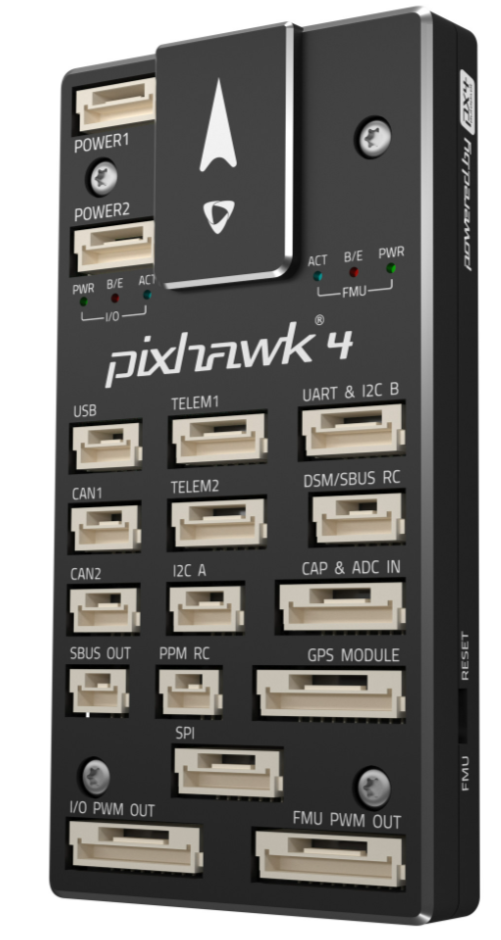
\includegraphics[scale=0.47]{obrazky/PIX}
    \end{center}
    \caption[Řídící jednotka Pixhawk 4]{Řídící jednotka Pixhawk 4 \cite{PX4docs}.}
    \label{fig:PIX}
\end{figure}

Mezi hlavní výhody řídících jednotek Pixhawk patří kvalitní softwarová podpora, automatické aktualizace firmware pomocí QGroundControl, flexibilita z hlediska připojených hardwarových periferií a silná komunita uživatelů a vývojářů. Jednotka Pixhawk podporuje aj simulaci \acs{HITL} (\textit{\acl{HITL}}), což umožňuje test firmwaru a komunikace ještě před samotným vzletem dronu.

\section{Palubní počítač}

Jako palubní počítač se na experimentální letecké mise využívá jednodeskový počítač Raspberry PI. Na trhu existuje množství různých variant tohoto široce rozšířeného počítače v rozmezí od levného, malého a úsporného  \textit{Raspberry PI Pico} až po vysoce výkonný počítač \textit{Raspberry PI 4B}.

Důležitými výhodami pro aplikace v robotických misích jsou integrace na jeden plošný spoj, nízká proudová spotřeba a možnost spuštění linuxových distribucí. Nejběžnější podporované distribuce jsou Raspberry PI OS, Raspbian, Ubuntu desktop a server.

Hlavní důvod pro použití Raspberry PI jako palubního počítače je možnost spolehlivé komunikace s PX4 firmware přes ROS 2 \textit{topic}. Komunikací mezi uvedenými platformami se budeme zabývat v následujících kapitolách

\section{Software pro řízení bezpilotních letadel}

Existují dvě hlavní větve vývoje firmware pro řídící jednotku Pixhawk. Jednou platformou je open source projekt ArduPilot \cite{ARDU}, který podporuje velké množství bezpilotních prostředků a umožňuje vytváření autonomních misí. Druhým projektem je profesionální autopilot PX4 \cite{PX4ORG}. Velkou výhodou obou projektů je, že jsou do velké části kompatibilní, například software pro pozemní stanice QGroundControl z platformy PX4 může komunikovat s řídící jednotkou s firmware od ArduPilot a naopak. Vzájemná kompatibilita je zajištěna využitím stejného komunikačního protokolu MAVLink. Výhoda protokolu MAVLink spočívá aj v tom, že oba firmware můžou komunikovat s ROS (Robot Operating System) přes MAVROS\footnote{MAVROS je komunikační ovládač (\textit{driver}) pro komunikaci mezi ROS a autopiloty s MAVLink protokolem}

\subsection{ArduPilot}

ArduPilot je open source autopilot podporující mnoho typů vozidel, například multikoptéry, tradiční vrtulníky, letadla s pevnými křídly, čluny, ponorky, rovery a další. Projekt ArduPilot má společnou historii s PX4, ale v minulosti se tyto dva projekty oddělili. Proto mají oba projekty do velké míry podobné využití a míří na stejnou platformu.

Zdrojový kód projektu ArduPilot je vyvíjen širokým spektrem profesionálů a nadšenců, takže výhodou je velká komunita poskytující řešení na řadu problémů.

Frimware ArduPilot je založený na ChibiOS \acs{RTOS} (\acl{RTOS}). ArduPilot taky poskytuje možnost simulace letového kódu jak simulací \acs{SITL} (\acl{SITL}), tak simulací \acs{HITL} (\acl{HITL}). \cite{ARDU}

Pro další pokračování v práci jsme zvolili projekt PX4, takže další části budou pojednávat už o firmware PX4.